% \setcounter{figure}{0}
% \setcounter{listing}{0}

\pagenumbering{arabic}
\renewcommand*{\thepage}{B-\arabic{page}}



\chapter{Description of Digital Submission \label{cha:cdrom} }

\textbf{Thesis Evidence Number:} \\ FIIT-182905-116308%\myEvidenceNumber
% \todo{nemam este evidencne cislo asi}

\textbf{Name of submitted archive:} \\
\texttt{DP\_MatejSevcik.zip}

The digital part included in the thesis contains the following files:

\begin{figure}[h]
    \begin{centering}
    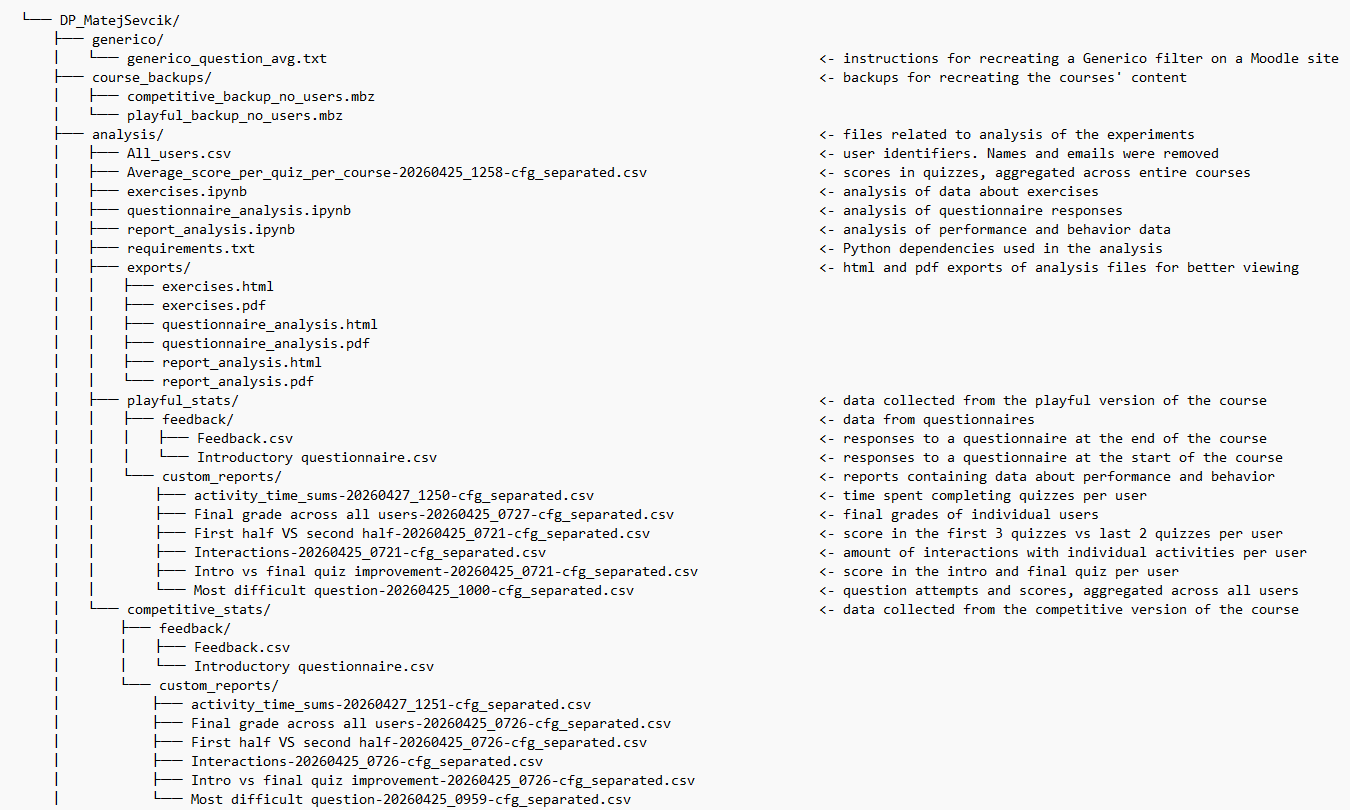
\includegraphics[width=\textwidth]{assets/images/installation/file_strucure_2_1.png}
    \par\end{centering}
\caption{The first half of the structure of the ZIP file \label{fig:zip-file-structure1}}
\end{figure}

\begin{figure}[h]
    \begin{centering}
    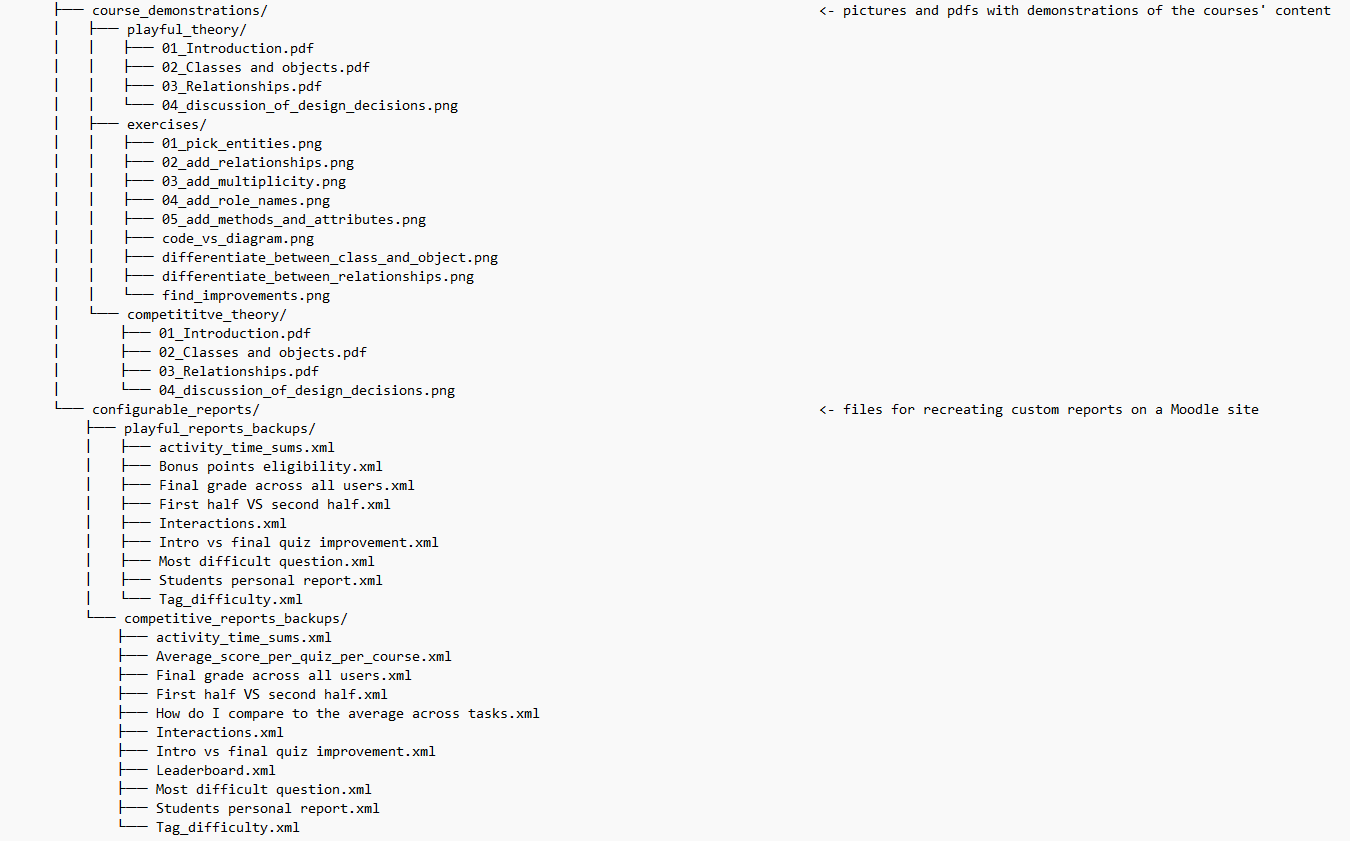
\includegraphics[width=\textwidth]{assets/images/installation/file_strucure_1_1.png}
    \par\end{centering}
\caption{The second half of the structure of the ZIP file \label{fig:zip-file-structure2}}
\end{figure}


\chapter{Technical Documentation}

\section{Installation Manual for Local Development}

The installation guide assumes the use of Windows 10 or 11 operating systems.

\begin{enumerate}
    \item Moodle provides installer packages for Windows that contain everything that is needed to run the application server locally. Download the latest stable release \href{https://download.moodle.org/windows/}{\color{blue}from the official website} (the version name should not end with dev. E.g. - instead of downloading \textit{Moodle 5.3dev}, download \textit{Moodle 5.2})
    \item Create a directory in a location where you want your local Moodle instance to reside
    \item Extract the installer package into the newly created directory
    \item Navigate to the extracted directory and run \texttt{Start Moodle.exe}
    \item Visit \href{http://localhost/}{\color{blue}http://localhost/} and follow displayed instructions to complete the installation
    \item \label{item:course-recreation} \texttt{(Optional)} If you want to recreate the courses used in this study: 
        \begin{enumerate}
            \item Log in as your admin user
            \item Install plugins according to instructions (Section~\ref{sec:plugin-installation})
            \item Navigate to \textbf{Site administration -> Courses -> Restore course} (\href{https://docs.moodle.org/502/en/Course_restore}{\color{blue}Course restore documentation})
            \item Drop one of the attached backups (\texttt{course\_backups/competitive\_backup\_no\_users.mbz} or \texttt{course\_backups/playful\_backup\_no\_users.mbz}) into the drop zone and click \textbf{Restore}. Do so for both attached courses individually
\begin{figure}[H]
\centering
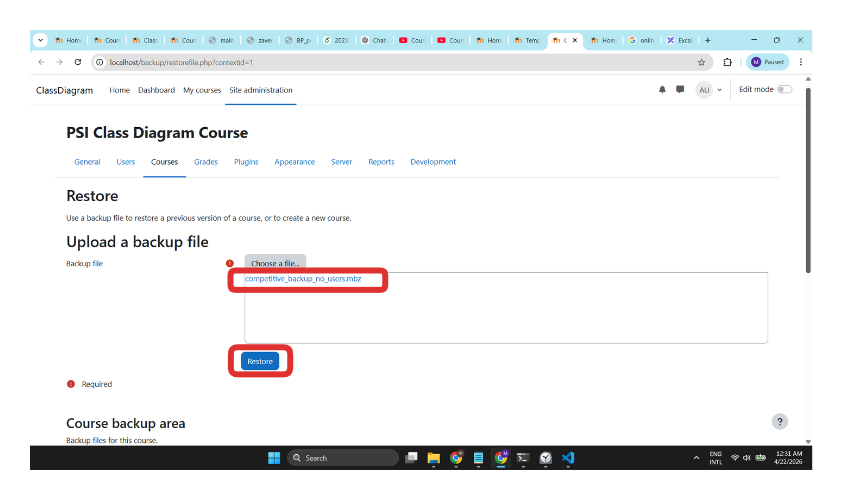
\includegraphics[width=0.8\textwidth]{assets/images/installation/course_restore_screen.png}
\caption{Restore a course from a backup in Moodle}
\label{fig:course-restore}
\end{figure}
            \item All the restore settings can be left at defaults. Pay care to select \textbf{Restore as new course} instead of \textbf{Restore into a course}
\begin{figure}[H]
\centering
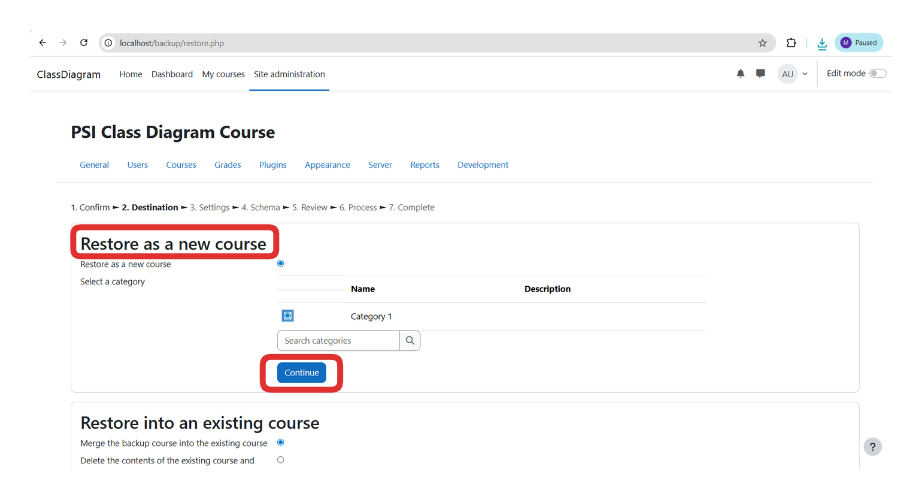
\includegraphics[width=0.8\textwidth]{assets/images/installation/restore_as_new_course.png}
\caption{Restore a backup as a new course}
\label{fig:restore-course-as-new-course}
\end{figure}
            \item Once the restore is pending, you need to run the cron task. On a production server, it runs automatically, but locally it must be executed manually from the command line. Open a terminal and run (the entire text is one command):
\begin{verbatim}
"<path-to-moodle>\server\php\php.exe"
"<path-to-moodle>\server\moodle\admin\cli\cron.php"
\end{verbatim}
        \end{enumerate}
\end{enumerate}


\section{Installation Manual for Production Environment}

\begin{enumerate}
    \item Obtain access to a Linux server (Recommended: Ubuntu 24.04.4 LTS)
    \item Set up the server according to \href{https://docs.moodle.org/500/en/}{\color{blue}instructions from Moodle documentation}
    \item \texttt{(Optional)} To recreate the courses used in this study, follow instructions from the previous section (item~\ref{item:course-recreation})
\end{enumerate}


\section{Plugin Installation} \label{sec:plugin-installation}

Plugins are not restored using course backups. Courses from this study work without plugins, but some of the e-learning features are not available without them. They are used for getting live statistics and reports. To recreate them, follow these instructions - they are the same for both production and local environments:

\begin{enumerate}
    \item Download plugins \href{https://moodle.org/plugins/filter_generico}{\color{blue}Generico filter} and \href{https://moodle.org/plugins/block_configurable_reports}{\color{blue}Configurable reports}
    \item Navigate to \textbf{Site administration -> Plugins -> Install plugins} (\href{https://docs.moodle.org/502/en/Installing_plugins}{\color{blue}Plugin installation documentation}). Drop the downloaded zip files into the displayed field and click \textbf{Install plugin from the ZIP file}
\begin{figure}[H]
\centering
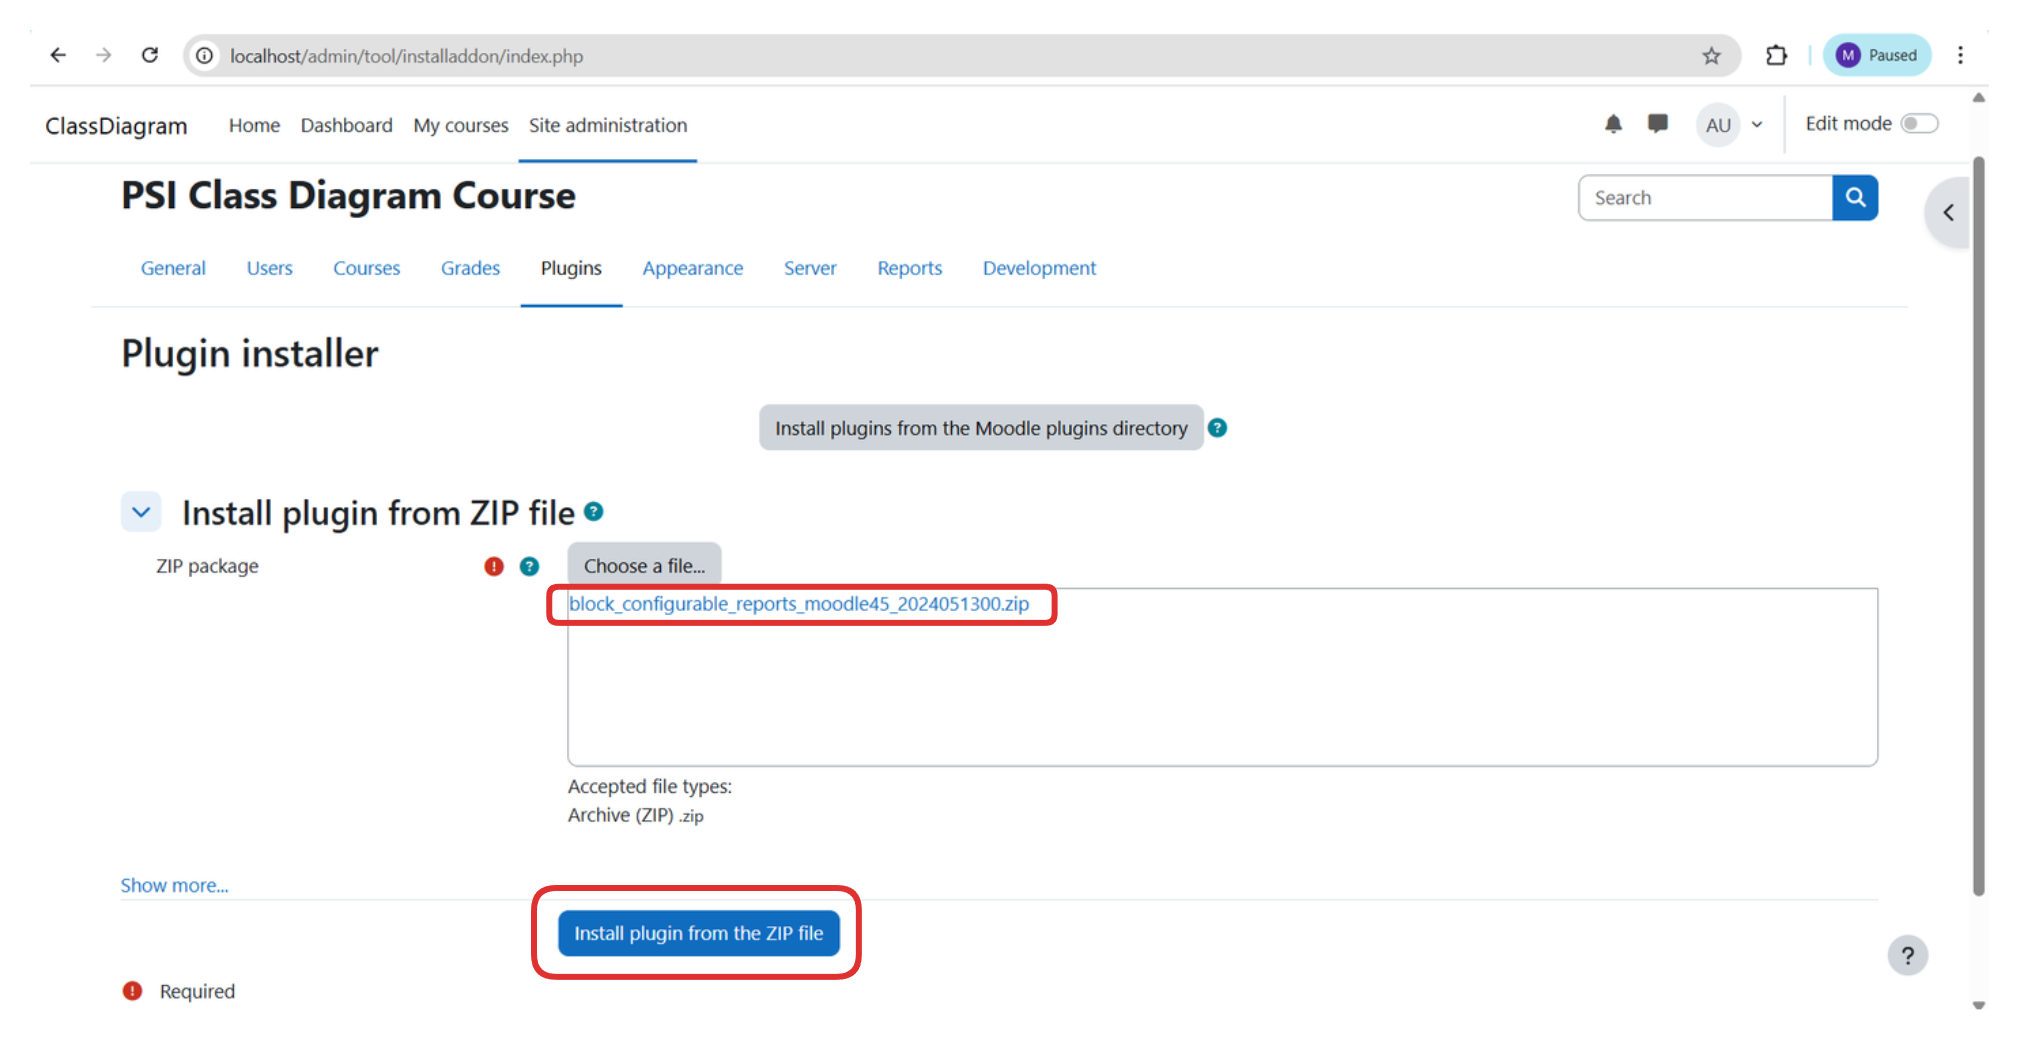
\includegraphics[width=0.8\textwidth]{assets/images/installation/plugin_installer.png}
\caption{Installing a plugin from a ZIP file in Moodle}
\label{fig:plugin-install}
\end{figure}
    \item \textbf{Configurable reports} 
        \begin{enumerate}
            \item Navigate to \textbf{<course-home>} side panel and go to \textbf{Configurable Reports -> Manage reports}
\begin{figure}[H]
\centering
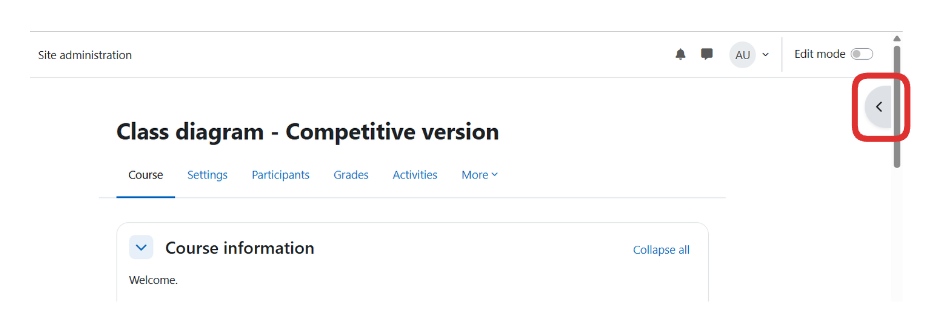
\includegraphics[width=0.8\textwidth]{assets/images/installation/Configurable_reports_nav_1.png}
\caption{Recreating Configurable reports in Moodle, step 1}
\label{fig:configurable-reports-1}
\end{figure}

\begin{figure}[H]
\centering
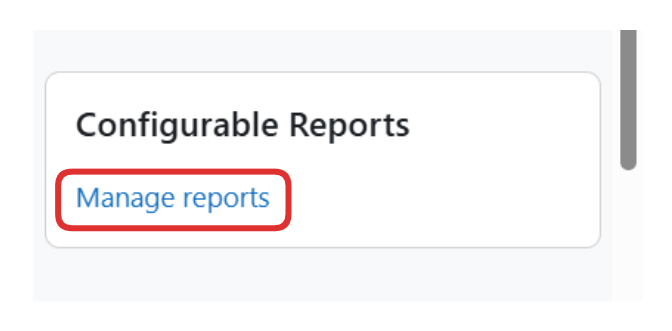
\includegraphics[width=0.8\textwidth]{assets/images/installation/Configurable_reports_nav_2.png}
\caption{Recreating Configurable reports in Moodle, step 2}
\label{fig:configurable-reports-2}
\end{figure}
            \item Drag each report backup (\texttt{configurable\_reports/competitive\_course\_backups/interactions.txt}) to the drop area in the corresponding course
    \begin{figure}[H]
\centering
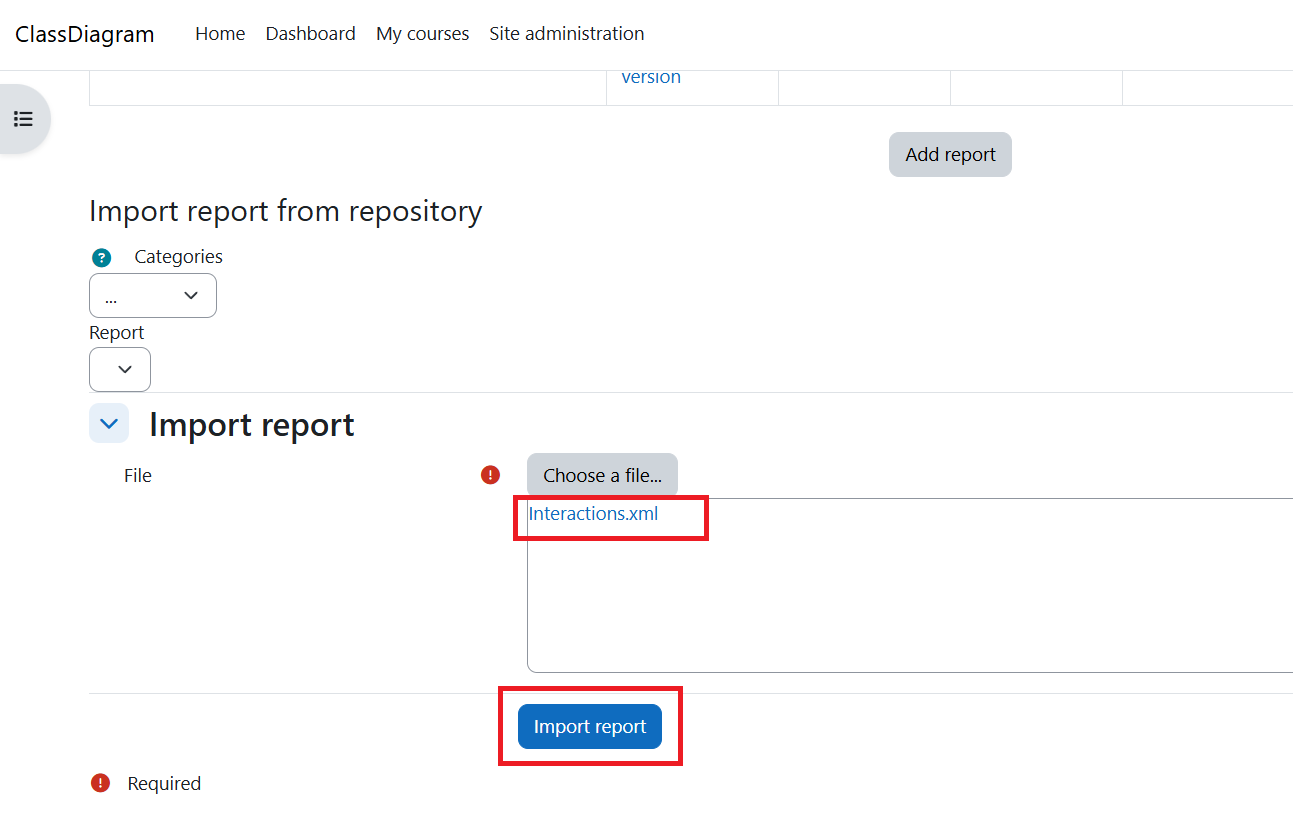
\includegraphics[width=0.8\textwidth]{assets/images/installation/Configurable_reports_nav_3.png}
\caption{Recreating Configurable reports in Moodle, step 3}
\label{fig:configurable-reports-3}
\end{figure}
        \end{enumerate}
    \item \textbf{Generico filter} 
        \begin{enumerate}
            \item Go to \textbf{Site administration -> Plugins -> Filters -> Category: Generico -> Templates} and click on one of the blank filters
\begin{figure}[H]
\centering
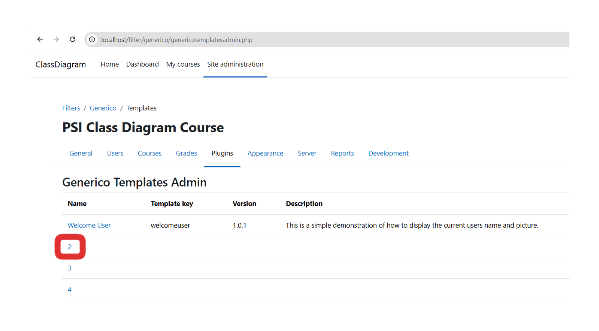
\includegraphics[width=0.8\textwidth]{assets/images/installation/generico.png}
\caption{Recreating a Generico filter in Moodle}
\label{fig:generico-nav}
\end{figure}
            \item copy values from \texttt{generico/generico\_question\_avg.txt} to their respective fields
            \item Each time the filter is used in the courses, the id in the filter is hardcoded. That means it needs to be manually updated in each instance (e.g. questions in the Competitve course contain \texttt{\{GENERICO:type=question\_avg,qid=507\}} in their descriptions - the id will need to be updated)
        \end{enumerate}
\end{enumerate}

% \section{User Guide for Teachers}

% -restore the course (same as local dev)
% -do i even include this part at all?
% -add students via csv? Do i have a reason to include that?
% -how to access the reports - custom and non custom? docs

% \section{Guide for Users (Students)}

% \begin{enumerate}
%     \item Log in using credentials received by email
%     \item 
% \end{enumerate}

% -create/obtain an account
% -fill out the course
% -some screenshots maybe?